\documentclass[12pt, titlepage]{article}

\usepackage{booktabs}
\usepackage{tabularx}
\usepackage{hyperref}
\hypersetup{
    colorlinks,
    citecolor=blue,
    filecolor=black,
    linkcolor=red,
    urlcolor=blue
}
\usepackage[round]{natbib}
\usepackage{graphicx}
\usepackage{caption}


%% Comments

\usepackage{color}

\newif\ifcomments\commentstrue %displays comments
%\newif\ifcomments\commentsfalse %so that comments do not display

\ifcomments
\newcommand{\authornote}[3]{\textcolor{#1}{[#3 ---#2]}}
\newcommand{\todo}[1]{\textcolor{red}{[TODO: #1]}}
\else
\newcommand{\authornote}[3]{}
\newcommand{\todo}[1]{}
\fi

\newcommand{\wss}[1]{\authornote{blue}{SS}{#1}} 
\newcommand{\plt}[1]{\authornote{magenta}{TPLT}{#1}} %For explanation of the template
\newcommand{\an}[1]{\authornote{cyan}{Author}{#1}}

%% Common Parts

\newcommand{\progname}{2D Localizer} % PUT YOUR PROGRAM NAME HERE
\newcommand{\authname}{Aliyah Jimoh} % AUTHOR NAMES                  

\usepackage{hyperref}
    \hypersetup{colorlinks=true, linkcolor=blue, citecolor=blue, filecolor=blue,
                urlcolor=blue, unicode=false}
    \urlstyle{same}
                                


\begin{document}

\title{System Verification and Validation Plan for 2D Localizer} 
\author{Aliyah Jimoh}
\date{\today}
	
\maketitle

\pagenumbering{roman}

\section*{Revision History}

\begin{tabularx}{\textwidth}{p{3cm}p{2cm}X}
\toprule {\bf Date} & {\bf Version} & {\bf Notes}\\
\midrule
24/02/2025 & 1.0 & Initial Draft\\
03/03/2025 & 1.1 & Feedback Implementation\\
\bottomrule
\end{tabularx}

~\\

\newpage

\tableofcontents

\listoftables

\listoffigures
\wss{Remove this section if it isn't needed}

\newpage

\section{Symbols, Abbreviations, and Acronyms}

\renewcommand{\arraystretch}{1.2}
\begin{tabular}{l l} 
  \toprule		
  \textbf{Symbol} & \textbf{Description}\\
  \midrule 
  2D & Two-Dimensional \\
  2D Localizer & 2D Localization Solution\\
  CRLB & Cram\'er-Rao Lower Bound\\
  FM & Fiducial Marker \\
  GTSAM & Georgia Tech Smoothing and Mapping\\
  MG & Module Guide \\
  MIS & Module Interface Specification \\
  MLE & Maximum Likelihood Estimation\\
  PEP8 & Python Enhancement Proposal 8 \\
  SE(2) & Special Euclidean Group in 2D \\
  SRS & Software Requirements Specification\\
  T & Test\\
  VnV & Verification and Validation\\
  \bottomrule
\end{tabular}\\

For a full list of symbols, abbreviations, and acronyms used, refer to section 1 in the \href{https://github.com/AliyahJimoh/2D-Localizer/blob/main/docs/SRS/SRS.pdf}{SRS} document.

\newpage

\pagenumbering{arabic}

This document shows the verification and validation plan of the 2D Localizer program. This plan starts with general information that talks about 2D Localizer in section \ref{sec_general}. The plan and system tests involved with this software is explained in sections \ref{sec_plan} and \ref{sec_sys-tests}.



\section{General Information}\label{sec_general}

\subsection{Summary}

This document examines the verification and validation plan of 2D Localizer. This software is used to help accurately locate mobile robots in a provided 2D map given the measurements and coordinates of the sensors and fiducial markers (FMs).

\subsection{Objectives}

The objective of this plan is to validate the accuracy of this program to build confidence in the software correctness. This plan also aims to satisfy all the requirements the System Requirements Specification (\href{https://github.com/AliyahJimoh/2D-Localizer/blob/main/docs/SRS/SRS.pdf}{SRS}) document outlined.  

% \wss{State what is intended to be accomplished.  The objective will be around
%   the qualities that are most important for your project.  You might have
%   something like: ``build confidence in the software correctness,''
%   ``demonstrate adequate usability.'' etc.  You won't list all of the qualities,
%   just those that are most important.}

% \wss{You should also list the objectives that are out of scope.  You don't have 
% the resources to do everything, so what will you be leaving out.  For instance, 
% if you are not going to verify the quality of usability, state this.  It is also 
% worthwhile to justify why the objectives are left out.}

% \wss{The objectives are important because they highlight that you are aware of 
% limitations in your resources for verification and validation.  You can't do everything, 
% so what are you going to prioritize?  As an example, if your system depends on an 
% external library, you can explicitly state that you will assume that external library 
% has already been verified by its implementation team.}

\subsection{Challenge Level and Extras}

This system has an advanced research level which can be seen from the implementation and the topic. Setting up the robot's movement, accurately displaying the trajectory, coordinating the sensors' measurements, and finding a way to animate the output would definitely add difficulty to this system, however, this is not a niche topic meaning that there are papers or libraries available to draw inspiration from.

% \wss{State the challenge level (advanced, general, basic) for your project.
% Your challenge level should exactly match what is included in your problem
% statement.  This should be the challenge level agreed on between you and the
% course instructor.  You can use a pull request to update your challenge level
% (in TeamComposition.csv or Repos.csv) if your plan changes as a result of the
% VnV planning exercise.}

% \wss{Summarize the extras (if any) that were tackled by this project.  Extras
% can include usability testing, code walkthroughs, user documentation, formal
% proof, GenderMag personas, Design Thinking, etc.  Extras should have already
% been approved by the course instructor as included in your problem statement.
% You can use a pull request to update your extras (in TeamComposition.csv or
% Repos.csv) if your plan changes as a result of the VnV planning exercise.}

\subsection{Relevant Documentation}

% \wss{Reference relevant documentation.  This will definitely include your SRS
%   and your other project documents (design documents, like MG, MIS, etc).  You
%   can include these even before they are written, since by the time the project
%   is done, they will be written.  You can create BibTeX entries for your
%   documents and within those entries include a hyperlink to the documents.}

% \citet{SRS}

% \wss{Don't just list the other documents.  You should explain why they are relevant and 
% how they relate to your VnV efforts.}

The documentation relevant to the 2D Localizer includes the Problem Statement since it explains the proposed software, the \href{https://github.com/AliyahJimoh/2D-Localizer/blob/main/docs/SRS/SRS.pdf}{SRS} which talks about the requirements needed to properly use the system, the Verification and Validation (\href{https://github.com/AliyahJimoh/2D-Localizer/blob/main/docs/VnVReport/VnVReport.pdf}{VnV}) report that goes through the tests and plans for the system, and the Module Guide (\href{https://github.com/AliyahJimoh/2D-Localizer/blob/main/docs/Design/SoftArchitecture/MG.pdf}{MG}) and Module Interface Specification (\href{https://github.com/AliyahJimoh/2D-Localizer/blob/main/docs/Design/SoftDetailedDes/MIS.pdf}{MIS}) for the design.

\section{Plan}\label{sec_plan}

This section describes the tests made for the 2D Localizer system. This begins by mentioning the VnV team in section~\ref{vnv_team}, then followed by the SRS Verification Plan in~\ref{plan_SRS}, the Design Verification Plan in section~\ref{plan_design},the VnV Plan Verification Plan in section~\ref{plan_verification}, the Implementation Verification Plan in section~\ref{plan_implement}, the Automated Testing and Verification tools in section~\ref{plan_auto}, and the Software Validation Plan in section~\ref{plan_software}.

\subsection{Verification and Validation Team}\label{vnv_team}

This section shows the members of the VnV team. They are shown in Table \ref{table:vnvTeam} along with what document they contributed in and their roles.

\begin{center}
  \begin{table}[h]
    \centering
    
    \begin{tabular}{|l|l|p{5cm}|}
        \hline
        \textbf{Name} & \textbf{Document} & \textbf{Role} \\
        \hline
        Aliyah Jimoh & All & Author\\
        \hline
        Dr.~Spencer Smith & All & Instructor \\
                          &     & Reviewer\\
        \hline
        Kiran Singh & SRS & Domain Expert\\
                    & VnV & Reviewer      \\
        \hline
        Dr.~Matthew Giamou & Problem Statement & Supervisor \\
                           &                   & Reviewer \\
        \hline
    \end{tabular}

    \caption{Verification and Validation Team}
    \label{table:vnvTeam}
\end{table}
\end{center}

\subsection{SRS Verification Plan}\label{plan_SRS}

The SRS document for 2D Localizer will be verified through the following steps:
\begin{enumerate}
  \item The initial review will be preformed by the assigned reviewers (Dr.~Spencer Smith and Kiran Singh) and will use the \href{https://github.com/AliyahJimoh/2D-Localizer/blob/main/docs/Checklists/SRS-Checklist.pdf}{SRS Checklist} as a guide.
  \item The reviewers will give feedback through creating issues in the GitHub repository.
  \item The author (Aliyah Jimoh) will apply the feedback to the document and address issues that may not be applied.
  \item The author will discuss with the supervisor (Dr.~Matthew Giamou) and ask for their input.
\end{enumerate}

% \wss{If you have a supervisor for the project, you shouldn't just say they will
% read over the SRS.  You should explain your structured approach to the review.
% Will you have a meeting?  What will you present?  What questions will you ask?
% Will you give them instructions for a task-based inspection?  Will you use your
% issue tracker?}

% \wss{Maybe create an SRS checklist?}

\subsection{Design Verification Plan}\label{plan_design}
The design for 2D Localizer will be verified through the following steps:
\begin{enumerate}
  \item The design documents, the MG and MIS, will be reviewed by the assigned reviewers (Kiran Singh and Dr.~Spencer Smith) and will use both checklists (\href{https://github.com/AliyahJimoh/2D-Localizer/blob/main/docs/Checklists/MG-Checklist.pdf}{MG Checklist} and \href{https://github.com/AliyahJimoh/2D-Localizer/blob/main/docs/Checklists/MIS-Checklist.pdf}{MIS Checklist}) as a guide.
  \item The reviewers will give feedback through creating issues in the GitHub repository.
  \item The author (Aliyah Jimoh) will apply the feedback to the document and address issues that may not be applied.
\end{enumerate}

% \wss{Plans for design verification}

% \wss{The review will include reviews by your classmates}

% \wss{Create a checklist?}

\subsection{Verification and Validation Plan Verification Plan}\label{plan_verification}

The VnV plan for 2D Localizer will be verified through the following steps:
\begin{enumerate}
  \item The VnV plan will be reviewed by the assigned reviewers (Kiran Singh and Dr.~Spencer Smith) and will use the \href{https://github.com/AliyahJimoh/2D-Localizer/blob/main/docs/Checklists/VnV-Checklist.pdf}{VnV Checklist} as a guide.
  \item The reviewers will give feedback through creating issues in the GitHub repository.
  \item The author (Aliyah Jimoh) will apply the feedback to the document and address issues that may not be applied.
\end{enumerate}

% \wss{The verification and validation plan is an artifact that should also be
% verified.  Techniques for this include review and mutation testing.}

% \wss{The review will include reviews by your classmates}

% \wss{Create a checklists?}

\subsection{Implementation Verification Plan}\label{plan_implement}

The implementation of 2D Localizer will be verified be the following techniques:
\begin{itemize}
  \item \textbf{Static Verification}
  \newline  
    The author will perform a code walkthrough the domain expert (Kiran Singh) and go through different tests to check the accuracy. The author will then do a walkthrough in a presentation while explaining the tests made and performed. 

  \item \textbf{Dynamic Testing}
  \newline
  The unit tests for 2D Localizer are discussed in section \ref{unit-test} 

\end{itemize}

% \wss{You should at least point to the tests listed in this document and the unit
%   testing plan.}

% \wss{In this section you would also give any details of any plans for static
%   verification of the implementation.  Potential techniques include code
%   walkthroughs, code inspection, static analyzers, etc.}

% \wss{The final class presentation in CAS 741 could be used as a code
% walkthrough.  There is also a possibility of using the final presentation (in
% CAS741) for a partial usability survey.}

\subsection{Automated Testing and Verification Tools}\label{plan_auto}

\subsubsection{Code Guidelines}
For Python implementation, the 2D Localization software will follow the coding style guidelines outlined in Python Enhancement Proposal 8 (PEP8). To enforce this, the Flake8 linter will be used to ensure that code meets PEP8's guidelines and for continuous integration in GitHub Actions.

\subsubsection{GTSAM Integration}
Georgia Tech Smoothing and Mapping (\href{https://github.com/borglab/gtsam}{GTSAM}) by~\cite{gtsam2022} is a library that implements sensor fusion for robotics using factor graphs. These graphs consist of two types of nodes: variables (e.g., robot poses and sensor measurements) and factors, which represent probabilistic constraints between them. 2D Localizer will be using this library as a modelling language and would need to run unit tests to verify if GTSAM is properly integrated.

\begin{figure}[h!]
  \begin{center}
    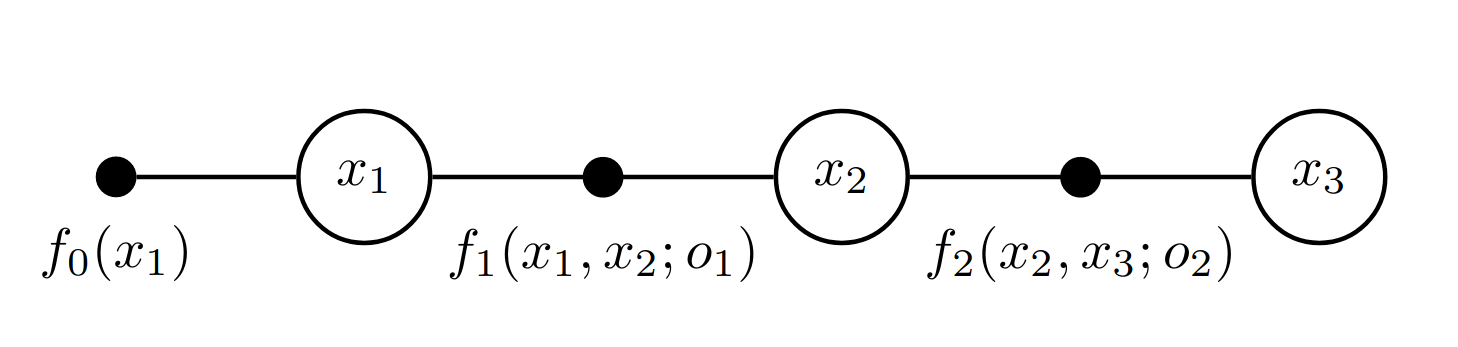
\includegraphics[width=0.6\textwidth]{factor_graph.png}
    \caption{Example Factor Graph from \cite{Dellaert2012}}
    \label{fig_factor} 
  \end{center}
\end{figure}

% \wss{What tools are you using for automated testing.  Likely a unit testing
%   framework and maybe a profiling tool, like ValGrind.  Other possible tools
%   include a static analyzer, make, continuous integration tools, test coverage
%   tools, etc.  Explain your plans for summarizing code coverage metrics.
%   Linters are another important class of tools.  For the programming language
%   you select, you should look at the available linters.  There may also be tools
%   that verify that coding standards have been respected, like flake9 for
%   Python.}

% \wss{If you have already done this in the development plan, you can point to
% that document.}

% \wss{The details of this section will likely evolve as you get closer to the
%   implementation.}

\subsection{Software Validation Plan}\label{plan_software}

To help validate the accuracy of the localization algorithm, 2D Localizer will use 2D data sets to test. If a data set cannot be found, alternative test cases and feedback will be discussed with the supervisor.

% \wss{If there is any external data that can be used for validation, you should
%   point to it here.  If there are no plans for validation, you should state that
%   here.}

% \wss{You might want to use review sessions with the stakeholder to check that
% the requirements document captures the right requirements.  Maybe task based
% inspection?}

% \wss{This section might reference back to the SRS verification section.}

\section{System Tests}\label{sec_sys-tests}

This section goes over the different system tests 2D Localizer will go through to satisfy its requirements.

% \wss{There should be text between all headings, even if it is just a roadmap of
% the contents of the subsections.}

\subsection{Tests for Functional Requirements}

% \wss{Subsets of the tests may be in related, so this section is divided into
%   different areas.  If there are no identifiable subsets for the tests, this
%   level of document structure can be removed.}

% \wss{Include a blurb here to explain why the subsections below
%   cover the requirements.  References to the SRS would be good here.}

This subsection looks at the system tests that will help satisfy the functional requirements outlined in the SRS (Section 5.1)

\subsubsection{Sensor Estimation Tests}

% \wss{It would be nice to have a blurb here to explain why the subsections below
%   cover the requirements.  References to the SRS would be good here.  If a section
%   covers tests for input constraints, you should reference the data constraints
%   table in the SRS.}

  These tests cover the requirements R1 to R3
		
\paragraph{Range-Only Pose Estimation}

\begin{enumerate}

\item{F-RO-01\\}

Control: Automatic
					
Initial State: 
\begin{itemize}
  \item Known beacon positions
  \item Robot starts at unknown location
\end{itemize}
					
Input: Range measurements $\tilde{d}_j$ from beacons with noise

Output: The estimated robot pose $\hat{x}$, as defined in the SRS (Section 5.1, Requirement R3).
 

Test Case Derivation: SRS Section IM2
					
How test will be performed: 
\begin{itemize}
  \item Use 2D dataset
  \item Run GTSAM-based factor graph optimization to estimate $\hat{x}$
  \item Verify the estimated error bounds align with FIM-derived uncertainty
\end{itemize}

\end{enumerate}


\paragraph{SE(2) Transformation Estimation}
\begin{enumerate}					
\item{F-SE2-01\\}

Control: Automatic
					
Initial State: 
\begin{itemize}
  \item Robot starts with a known pose $T_{wf}$
  \item Fiducial markers are placed at fixed positions
\end{itemize}
					
Input: Transformation matrices $T_{wf}, T_{br}$ 

Output: Computed transformation must satisfy:
\[
T_{wr} = T_{wf} T_{fr}
\]

Test Case Derivation: The transformation matrix $T_{wr}$ is computed using the rigid-body transformation rule in SE(2), which is required to maintain the system’s geometric consistency (SRS Section TM3)

How test will be performed: 
\begin{itemize}
  \item Compute $T_{wr}$ using both analytical and numerical methods
  \item Compare GTSAM-computed pose with theoretical SE(2) output
\end{itemize}
\end{enumerate}

\paragraph{Range + SE(2) Sensor Fusion Test}
\begin{enumerate}
\item{F-SF-01\\}

Control: Automatic
					
Initial State: 
\begin{itemize}
  \item Robot starts at unknown pose
  \item Beacons and fiducial markers placed in test environment
\end{itemize}
					
Input: Range measurements + SE(2) transformation constraints

Output: Estimated pose $T_{wr}$ and $\hat{x}$

Test Case Derivation: F-RO-01 and F-SE2-01

How test will be performed: 
\begin{itemize}
  \item Construct factor graph in GTSAM
  \item Run optimization twice (once with range only, once with full fusion)
  \item Compare error reductions
\end{itemize}

\end{enumerate}

\subsubsection{Visual Testing}
This test covers the requirement R5

\paragraph{2D Map Overlay of Estimated Poses}
\begin{enumerate}					
\item{F-MO-01\\}

Control: Automatic
					
Initial State: 
\begin{itemize}
  \item Environment 2D map and sensor locations (beacons, fiducials) are known.
  \item Robot follows a predefined trajectory.
\end{itemize}
					
Input: \begin{itemize}
  \item Ground truth trajectory $T_{wr}$
  \item Estimated trajectory from localization output $\hat{x}$, generated by a GTSAM-based factor graph optimization.
  \item Sensor positions and detections.
\end{itemize}

Output: The visualization correctly displays:
\begin{itemize}
    \item Estimated trajectory $\hat{x}$ based on GTSAM’s factor graph optimization.
    \item Sensor placements (beacons, fiducial markers).
\end{itemize}

Test Case Derivation: The estimated pose $\hat{x}$ is computed using Maximum Likelihood Estimation (MLE), as described in SRS Section IM2.

How test will be performed: 
\begin{itemize}
  \item Run GTSAM-based localization and extract optimized poses $\hat{x}$.
  \item Generate a visualization overlaying $\hat{x}$ on the environment map.
  \item Compare the generated visualization with an expected ground-truth image.
\end{itemize}

\end{enumerate}

\subsection{Tests for Nonfunctional Requirements}

% \wss{The nonfunctional requirements for accuracy will likely just reference the
%   appropriate functional tests from above.  The test cases should mention
%   reporting the relative error for these tests.  Not all projects will
%   necessarily have nonfunctional requirements related to accuracy.}

% \wss{For some nonfunctional tests, you won't be setting a target threshold for
% passing the test, but rather describing the experiment you will do to measure
% the quality for different inputs.  For instance, you could measure speed versus
% the problem size.  The output of the test isn't pass/fail, but rather a summary
% table or graph.}

% \wss{Tests related to usability could include conducting a usability test and
%   survey.  The survey will be in the Appendix.}

% \wss{Static tests, review, inspections, and walkthroughs, will not follow the
% format for the tests given below.}

% \wss{If you introduce static tests in your plan, you need to provide details.
% How will they be done?  In cases like code (or document) walkthroughs, who will
% be involved? Be specific.}

\subsubsection{Estimation Accuracy}
		
\paragraph{Accuracy Validation}

\begin{enumerate}

\item{NF-ACC-01\\}

Type: Nonfunctional, Dynamic, Automatic
					
Initial State: 
\begin{itemize}
  \item The system has access to ground truth robot poses $\bar{x}$.
  \item Sensor measurements (range, fiducial marker detections) are available.
\end{itemize}
					
Input/Condition: 
\begin{itemize}
  \item Synthetic and real-world sensor data.
  \item Estimated robot poses $\hat{x}$, generated using a GTSAM-based factor graph optimization.
  \item Ground truth robot trajectory.
\end{itemize}
					
Output/Result: 
\begin{itemize}
  \item The Root Mean Squared Error (RMSE) of the estimated poses $\hat{x}$ must satisfy the accuracy constraint in SRS Section 5.2, Requirement NFR1.
  \item The estimated pose covariance must not exceed the theoretical Cram\'er-Rao Lower Bound (CRLB) (SRS Section TM2).
\end{itemize}
					
How test will be performed: 
\begin{itemize}
  \item Generate test cases with ground-truth trajectory $\bar{x}$.
  \item Compute estimated poses $\hat{x}$ using GTSAM factor graph optimization.
  \item Evaluate RMSE between $\hat{x}$ and $\bar{x}$:
  \item Compare estimated variance to the CRLB (TM3)
\end{itemize}

\end{enumerate}

\newpage
\subsection{Traceability Between Test Cases and Requirements}

\begin{table}[h!]
  \centering
  \begin{tabular}{|c|c|c|c|c|c|}
  \hline
    & F-RO-01 & F-SE2-01 & F-SF-01 & F-MO-01 & NF-ACC-01 \\
  \hline
  R1          &X &X &X & X& \\ \hline
  R2           &X & &X & &X \\ \hline
  R3         &X & &X & & \\ \hline
  R4   & & & & & \\ \hline
  R5      & & & &X & \\
  \hline
  \end{tabular}
  \caption{Traceability Matrix Showing the Connections Between Requirements and System Tests}
\end{table}


\section{Unit Test Description}\label{unit-test}

\wss{This section should not be filled in until after the MIS (detailed design
  document) has been completed.}

\wss{Reference your MIS (detailed design document) and explain your overall
philosophy for test case selection.}  

\wss{To save space and time, it may be an option to provide less detail in this section.  
For the unit tests you can potentially layout your testing strategy here.  That is, you 
can explain how tests will be selected for each module.  For instance, your test building 
approach could be test cases for each access program, including one test for normal behaviour 
and as many tests as needed for edge cases.  Rather than create the details of the input 
and output here, you could point to the unit testing code.  For this to work, you code 
needs to be well-documented, with meaningful names for all of the tests.}

\subsection{Unit Testing Scope}

\wss{What modules are outside of the scope.  If there are modules that are
  developed by someone else, then you would say here if you aren't planning on
  verifying them.  There may also be modules that are part of your software, but
  have a lower priority for verification than others.  If this is the case,
  explain your rationale for the ranking of module importance.}

\subsection{Tests for Functional Requirements}

\wss{Most of the verification will be through automated unit testing.  If
  appropriate specific modules can be verified by a non-testing based
  technique.  That can also be documented in this section.}

\subsubsection{Module 1}

\wss{Include a blurb here to explain why the subsections below cover the module.
  References to the MIS would be good.  You will want tests from a black box
  perspective and from a white box perspective.  Explain to the reader how the
  tests were selected.}

\begin{enumerate}

\item{test-id1\\}

Type: \wss{Functional, Dynamic, Manual, Automatic, Static etc. Most will
  be automatic}
					
Initial State: 
					
Input: 
					
Output: \wss{The expected result for the given inputs}

Test Case Derivation: \wss{Justify the expected value given in the Output field}

How test will be performed: 
					
\item{test-id2\\}

Type: \wss{Functional, Dynamic, Manual, Automatic, Static etc. Most will
  be automatic}
					
Initial State: 
					
Input: 
					
Output: \wss{The expected result for the given inputs}

Test Case Derivation: \wss{Justify the expected value given in the Output field}

How test will be performed: 

\item{...\\}
    
\end{enumerate}

\subsubsection{Module 2}

...

\subsection{Tests for Nonfunctional Requirements}

\wss{If there is a module that needs to be independently assessed for
  performance, those test cases can go here.  In some projects, planning for
  nonfunctional tests of units will not be that relevant.}

\wss{These tests may involve collecting performance data from previously
  mentioned functional tests.}

\subsubsection{Module ?}
		
\begin{enumerate}

\item{test-id1\\}

Type: \wss{Functional, Dynamic, Manual, Automatic, Static etc. Most will
  be automatic}
					
Initial State: 
					
Input/Condition: 
					
Output/Result: 
					
How test will be performed: 
					
\item{test-id2\\}

Type: Functional, Dynamic, Manual, Static etc.
					
Initial State: 
					
Input: 
					
Output: 
					
How test will be performed: 

\end{enumerate}

\subsubsection{Module ?}

...

\subsection{Traceability Between Test Cases and Modules}

\wss{Provide evidence that all of the modules have been considered.}

				
\bibliographystyle{plainnat}

\bibliography{../../refs/References}

\newpage

\section{Appendix}\label{sec_appendix}

This is where you can place additional information.

\subsection{Symbolic Parameters}

The definition of the test cases will call for SYMBOLIC\_CONSTANTS.
Their values are defined in this section for easy maintenance.

\subsection{Usability Survey Questions?}

\wss{This is a section that would be appropriate for some projects.}

\newpage{}

\end{document}